% Options for packages loaded elsewhere
\PassOptionsToPackage{unicode}{hyperref}
\PassOptionsToPackage{hyphens}{url}
%
\documentclass[
]{article}
\author{}
\date{}

\usepackage{amsmath,amssymb}
\usepackage{booktabs}
\usepackage{lmodern}
\usepackage{iftex}
\usepackage{siunitx}
\usepackage{pgfplots}
\ifPDFTeX
  \usepackage[T1]{fontenc}
  \usepackage[utf8]{inputenc}
  \usepackage{textcomp} % provide euro and other symbols
\else % if luatex or xetex
  \usepackage{unicode-math}
  \defaultfontfeatures{Scale=MatchLowercase}
  \defaultfontfeatures[\rmfamily]{Ligatures=TeX,Scale=1}
\fi
% Use upquote if available, for straight quotes in verbatim environments
\IfFileExists{upquote.sty}{\usepackage{upquote}}{}
\IfFileExists{microtype.sty}{% use microtype if available
  \usepackage[]{microtype}
  \UseMicrotypeSet[protrusion]{basicmath} % disable protrusion for tt fonts
}{}
\makeatletter
\@ifundefined{KOMAClassName}{% if non-KOMA class
  \IfFileExists{parskip.sty}{%
    \usepackage{parskip}
  }{% else
    \setlength{\parindent}{0pt}
    \setlength{\parskip}{6pt plus 2pt minus 1pt}}
}{% if KOMA class
  \KOMAoptions{parskip=half}}
\makeatother
\usepackage{xcolor}
\IfFileExists{xurl.sty}{\usepackage{xurl}}{} % add URL line breaks if available

\urlstyle{same} % disable monospaced font for URLs
\usepackage{color}
\usepackage{fancyvrb}
\usepackage[
    backend=biber,
    style=ieee,
    citestyle=ieee,
    % defernumbers=true
]{biblatex}
\addbibresource{pascal.bib}

\usepackage{hyperref}
\usepackage{cleveref}
\hypersetup{
  hidelinks,
  pdfcreator={LaTeX}}
\newcommand{\VerbBar}{|}
\newcommand{\VERB}{\Verb[commandchars=\\\{\}]}
\DefineVerbatimEnvironment{Highlighting}{Verbatim}{commandchars=\\\{\}}
% Add ',fontsize=\small' for more characters per line
\newenvironment{Shaded}{}{}
\newcommand{\AlertTok}[1]{\textcolor[rgb]{1.00,0.00,0.00}{\textbf{#1}}}
\newcommand{\AnnotationTok}[1]{\textcolor[rgb]{0.38,0.63,0.69}{\textbf{\textit{#1}}}}
\newcommand{\AttributeTok}[1]{\textcolor[rgb]{0.49,0.56,0.16}{#1}}
\newcommand{\BaseNTok}[1]{\textcolor[rgb]{0.25,0.63,0.44}{#1}}
\newcommand{\BuiltInTok}[1]{#1}
\newcommand{\CharTok}[1]{\textcolor[rgb]{0.25,0.44,0.63}{#1}}
\newcommand{\CommentTok}[1]{\textcolor[rgb]{0.38,0.63,0.69}{\textit{#1}}}
\newcommand{\CommentVarTok}[1]{\textcolor[rgb]{0.38,0.63,0.69}{\textbf{\textit{#1}}}}
\newcommand{\ConstantTok}[1]{\textcolor[rgb]{0.53,0.00,0.00}{#1}}
\newcommand{\ControlFlowTok}[1]{\textcolor[rgb]{0.00,0.44,0.13}{\textbf{#1}}}
\newcommand{\DataTypeTok}[1]{\textcolor[rgb]{0.56,0.13,0.00}{#1}}
\newcommand{\DecValTok}[1]{\textcolor[rgb]{0.25,0.63,0.44}{#1}}
\newcommand{\DocumentationTok}[1]{\textcolor[rgb]{0.73,0.13,0.13}{\textit{#1}}}
\newcommand{\ErrorTok}[1]{\textcolor[rgb]{1.00,0.00,0.00}{\textbf{#1}}}
\newcommand{\ExtensionTok}[1]{#1}
\newcommand{\FloatTok}[1]{\textcolor[rgb]{0.25,0.63,0.44}{#1}}
\newcommand{\FunctionTok}[1]{\textcolor[rgb]{0.02,0.16,0.49}{#1}}
\newcommand{\ImportTok}[1]{#1}
\newcommand{\InformationTok}[1]{\textcolor[rgb]{0.38,0.63,0.69}{\textbf{\textit{#1}}}}
\newcommand{\KeywordTok}[1]{\textcolor[rgb]{0.00,0.44,0.13}{\textbf{#1}}}
\newcommand{\NormalTok}[1]{#1}
\newcommand{\OperatorTok}[1]{\textcolor[rgb]{0.40,0.40,0.40}{#1}}
\newcommand{\OtherTok}[1]{\textcolor[rgb]{0.00,0.44,0.13}{#1}}
\newcommand{\PreprocessorTok}[1]{\textcolor[rgb]{0.74,0.48,0.00}{#1}}
\newcommand{\RegionMarkerTok}[1]{#1}
\newcommand{\SpecialCharTok}[1]{\textcolor[rgb]{0.25,0.44,0.63}{#1}}
\newcommand{\SpecialStringTok}[1]{\textcolor[rgb]{0.73,0.40,0.53}{#1}}
\newcommand{\StringTok}[1]{\textcolor[rgb]{0.25,0.44,0.63}{#1}}
\newcommand{\VariableTok}[1]{\textcolor[rgb]{0.10,0.09,0.49}{#1}}
\newcommand{\VerbatimStringTok}[1]{\textcolor[rgb]{0.25,0.44,0.63}{#1}}
\newcommand{\WarningTok}[1]{\textcolor[rgb]{0.38,0.63,0.69}{\textbf{\textit{#1}}}}
\setlength{\emergencystretch}{3em} % prevent overfull lines
\providecommand{\tightlist}{%
  \setlength{\itemsep}{0pt}\setlength{\parskip}{0pt}}
\setcounter{secnumdepth}{-\maxdimen} % remove section numbering
\ifLuaTeX
  \usepackage{selnolig}  % disable illegal ligatures
\fi


\begin{document}

\section{Encoder Implementation}\label{encoder-implementation}

Existing literature~\cite{Lengerke2022,Lengerke2023,Ferrara2022} has developed reed-salomon (RS) codes as an ID
code with great statistical properties. However, the encoding time of
the surveyed RS implementations is orders of magnitude slower than industry standard hashing functions like Sha2~\cite{Lengerke2022,Ferrara2022}. As a result practical applications are limited.

\cite{Ferrara2022} demonstrates significantly improved encoding speeds by using binary extension fields. However, the presented implementation only reached speeds of $10Mbits/s = 1.22MiB/s$. Those speeds are still far slower than Sha2 which can reach speeds of $2.25GiB/s$ (see \cref{sec:bench}). Furthermore, the presented speed implementation is limited to a small field size of $2^{8}$ which significantly limits the world size. Henceforth, an alternative encoder implementation is described which can reach similar throughput as Sha2 while also allowing significantly larger fields/world sizes.

An RS encoder operates on a list of symbols \(s_i\). These symbols are
elements of finite field \(s_i \in GF(n)\). The resulting RS code
(usually) has \(n - 1\) symbols \(r_j\) that are obtained by multiplying
each element with a power of the fields' generator \(a\). A generator
\(a \in GF(n)\) is a finite field element whose powers
 are all unique \(a^i \neq a^j \quad 0 \le i, j \le n - 1\). The symbols of the RS
code can be calculated with

\begin{equation}
r_j = \sum_{i=0}^{n - 1} s_i a^{j i}.
\end{equation}

For an ID code only one (random) symbol $r_j$ needs to be computed.

 In literature prime fields are usually used for RS-ID encoders~\cite{Lengerke2022,Lengerke2023}. These
are fields where \(n\) is a prime number. These fields are isomorphic to
the ring of integers modulus \(n\): \(GF(n) \cong \mathbb{Z} / n\mathbb{Z}\).
Therefore, multiplication is fairly fast as the CPU can just perform
normal integer multiplication and calculate the remainder afterwards (so
multiplication is only twice as slow as normal multiplication). However,
computer memory is encoded as bytes. Converting that memory to prime requires treating that memory as  variable sized integer and performing a radix conversion. This conversion essentially involves repeated division/remainder calculation. As big integer division has linear time complexity $O(N)$, this radix conversion has time complexity of \(O(n^2)\) (with a high time factor).

\newpage
\subsection{(Binary) Extension Field
Construction}\label{binary-extension-field-construction}

Other established applications of RS encoding (and finite fields in
general) such as RAID-6 therefore use (binary) extension fields instead. This approach is also used in~\cite{Ferrara2022}.
Extension fields are finite fields with the cardinality of a prime power
\(n = p^z\). The elements of such a field are polynomials of degree
\(z - 1\) with coefficients in its base prime field:

\begin{equation}
b = b_{z - 1} x^{z - 1} + .. + b_1 x + b_0 \quad b \in GF(p^z), b_i \in GF(p).
\end{equation}

Addition/Subtraction of polynomials is simply performed element wise.
For binary extension fields in particular both addition and subtraction
are equivalent to XOR. Polynomial multiplication can create
elements outside the finite field. For example:

\begin{equation}
x^{2z - 2} = x^{z - 1} x^{z - 1} \notin GF(p^z).
\end{equation}

To construct an extension field it is necessary to select an irreducible
rank \(z\) polynomial \(P\). Multiplication in
the extension field is then defined as polynomial multiplication modulus
\(P\). A field constructed this way retains all properties of prime
fields.

Binary extension fields (\(p = 2\)) are of particular interest because
their elements can be represented by binary numbers of length \(z\). If
z is a (power of two) multiple of 8 then symbols correspond to
bytes/words which can be read directly from memory without additional
overhead (and are well suited for processing with CPU instructions).

\subsection{Binary Extension Field
Implementation}\label{binary-extension-field-implementation}

As previously mentioned addition and subtraction of binary extension
fields can be implemented using a XOR. For small fields ($GF(2^{8}$) and
$GF(2^{16})$)  multiplication can be implemented using a lookup table (LUT). Here the
g2p~\cite{Wanzenbock} library was used. However, an LUT based apporach become impractically
large for higher \(z\) (like $GF(2^{32})$) as it has a space complexity of $O(n^2)$.

Efficient multiplication of 32bit and 64bit finite fields can be implemented using
carryless multiply instruction sets insted. These instructions are available on all amd64 CPUs released since 2011 and on all aarch64 CPUs. Carryless
multiply (CLMU) instructions perform a simple polynomial multiplication
(without a modulus) as described in~\cref{binary-extension-field-construction}. The 32/64
bit modulus of the resulting 64/128 bit polynomial can be computed by
utilizing the CLMU instruction to perform a barrett reduction as
described in~\cite{Dixon2009}. A practical
implementation is slightly more involved as implementing the bit
shuffling can be complex. An implementation of a 32 bit for amd64 is shown below.

\begin{Shaded}
\begin{Highlighting}[]
\KeywordTok{fn}\NormalTok{ barrett\_reduce(x}\OperatorTok{:} \NormalTok{\_\_m128i) }\OperatorTok{{-}\textgreater{}} \DataTypeTok{u32} \OperatorTok{\{}
    \KeywordTok{let}\NormalTok{ pu }\OperatorTok{=} \NormalTok{\_mm\_set\_epi64x(U\_PRIME}\OperatorTok{,}\NormalTok{ P\_X)}\OperatorTok{;}
    \KeywordTok{let}\NormalTok{ t1 }\OperatorTok{=} \NormalTok{\_mm\_clmulepi64\_si128(}
        \NormalTok{\_mm\_and\_si128(x}\OperatorTok{,} \NormalTok{\_mm\_set\_epi32(}\DecValTok{0}\OperatorTok{,} \DecValTok{0}\OperatorTok{,} \OperatorTok{!}\DecValTok{0}\OperatorTok{,} \DecValTok{0}\NormalTok{))}\OperatorTok{,}
\NormalTok{        pu}\OperatorTok{,}
        \DecValTok{0x10}\OperatorTok{,}
\NormalTok{    )}\OperatorTok{;}
    \KeywordTok{let}\NormalTok{ t2 }\OperatorTok{=} \NormalTok{\_mm\_clmulepi64\_si128(}
        \NormalTok{\_mm\_and\_si128(t1}\OperatorTok{,} \NormalTok{\_mm\_set\_epi32(}\DecValTok{0}\OperatorTok{,} \OperatorTok{!}\DecValTok{0}\OperatorTok{,} \DecValTok{0}\OperatorTok{,} \DecValTok{0}\NormalTok{))}\OperatorTok{,}
\NormalTok{        pu}\OperatorTok{,}
        \DecValTok{0x01}\OperatorTok{,}
\NormalTok{    )}\OperatorTok{;}

    \KeywordTok{let}\NormalTok{ tmp }\OperatorTok{=} \NormalTok{\_mm\_extract\_epi32(t2}\OperatorTok{,} \DecValTok{0}\NormalTok{) }\KeywordTok{as} \DataTypeTok{u32}\OperatorTok{;}
    \KeywordTok{let}\NormalTok{ x }\OperatorTok{=} \NormalTok{\_mm\_extract\_epi32(x}\OperatorTok{,} \DecValTok{0}\NormalTok{) }\KeywordTok{as} \DataTypeTok{u32}\OperatorTok{;}

\NormalTok{    tmp }\OperatorTok{\^{}}\NormalTok{ x}
\OperatorTok{\}}
\end{Highlighting}
\end{Shaded}

Computing powers by naively repeating multiplication is very slow.
Instead, the square-and-multiply implementation from the g2p library~\cite{Wanzenbock} is used here. The performance of the implementation isn't critical as an
efficient RS-ID encoder only needs to compute a single power (see \cref{simple-rs-id-encoder-implementation}).

\subsection{Simple RS-ID encoder
implementation}\label{simple-rs-id-encoder-implementation}

For a binary extension field \(GF(2^z)\) where \(z=8*2^l\) the input
symbols can simply directly read from memory (assuming its sufficiently
aligned). If T is an integer with the size of the symbol then such a RS
encoder can be implemented as follows (all arithmetic is performed in
the finite field):

\begin{Shaded}
\begin{Highlighting}[]
\KeywordTok{fn}\NormalTok{ encode\_rs(data}\OperatorTok{:} \OperatorTok{\&}\NormalTok{[T]}\OperatorTok{,}\NormalTok{ cue}\OperatorTok{:} \DataTypeTok{usize}\NormalTok{) }\OperatorTok{{-}\textgreater{}}\NormalTok{ T }\OperatorTok{\{}
    \KeywordTok{if}\NormalTok{ data}\OperatorTok{.}\NormalTok{is\_empty() }\OperatorTok{\{}
        \KeywordTok{return}\NormalTok{ zero()}\OperatorTok{;}
    \OperatorTok{\}}
    \KeywordTok{let} \KeywordTok{mut}\NormalTok{ res }\OperatorTok{=}\NormalTok{ data[}\DecValTok{0}\NormalTok{]}\OperatorTok{;}
    \KeywordTok{let}\NormalTok{ initial\_generator }\OperatorTok{=}\NormalTok{ GENERATOR}\OperatorTok{.}\NormalTok{pow(cue)}\OperatorTok{;}
    \KeywordTok{let} \KeywordTok{mut}\NormalTok{ generator }\OperatorTok{=}\NormalTok{ initial\_generator}\OperatorTok{;}
    \KeywordTok{for}\NormalTok{ symbol }\KeywordTok{in}\NormalTok{ data[}\DecValTok{1}\OperatorTok{..}\NormalTok{] }\OperatorTok{\{}
\NormalTok{        res }\OperatorTok{+=}\NormalTok{ generator }\OperatorTok{*}\NormalTok{ symbol}\OperatorTok{;}
\NormalTok{        generator }\OperatorTok{*=}\NormalTok{ initial\_generator}\OperatorTok{;}
    \OperatorTok{\}}
\NormalTok{    res}
\OperatorTok{\}}
\end{Highlighting}
\end{Shaded}

\pagebreak
Compared to a more naive implementation the input data is not zero
padded. For the zero symbol \(s_i a^{j i} = 0\) always holds. The zero
padded symbols therefore never contribute anything to the final sum.
Furthermore, the generator power is not recomputed in each loop
iteration. Instead, the generator power for the next iteration is
calculated at the end of every iteration:
\(a^{j (i + 1)} = a^{j i} a^{j}\). This optimization alone allowed a
speedup by a factor of 64.

\subsection{Optimized 32 bit and 64 RS-ID encoder
implementation}\label{optimized-32-bit-rs-id-encoder-implementation}

CPUs usually only implement a single 64 bit CLMU instruction with a 128
bit output register. This fact can be used to optimize the 32 bit and 64 bit RS
encoder even further. The barrett reduction introduced in~\cite{Dixon2009}
requires two CLMU instructions and many additional instructions for bit
shuffling and is therefore much slower than the main CLMU.

The distributive and associative properties of the modulus
operation~\cite{Dixon2009} shown in \eqref{eq:modmul} and \eqref{eq:modsum} can be used to avoid almost all barrett reductions and therefore significantly speed up the encoder.
  
\begin{gather}
\begin{gathered}
(f \mod P) \otimes (g \mod P) \mod P = f \otimes (g \mod P) \mod P\\
= (f \mod P) \otimes g \mod P = f \otimes g \mod P\\
\end{gathered}\label{eq:modmul}\\
\begin{gathered}
(f \mod P) \oplus (g  \mod P) \mod P = f \oplus (g \mod P) \mod P\\
 = (f \mod P) \oplus g \mod P = f \oplus g \mod P\label{eq:modsum}
\end{gathered}
\end{gather}

Note that \eqref{eq:modmul} only holds on hardware as long as the register is large enough
to hold the result. That means that at most three 32bit elements and two 64 bit elements can be
multiplied before a reduction is necessary. However, an unlimited number
of elements can be added without requiring reduction as polynomial addition cannot overflow. Therefore, all products of the RS computation can be summed without performing a barrett
reduction. Only a single barrett reduction of the final sum is necessary.

However, the exponent of the generator \(a^{ji + 1} = a^{ji} a^j\) still
requires a barrett reduction for every element as the product would
quickly exceed the register size. The cost of this barrett reduction can
be amortized by splitting input symbols into shards of
length \(m\) that are encoded individually:

\begin{gather}
R_{j,k} = \sum_l^m a^{jl} s_{k*m+l}\\
r_j = \sum_k^{n/m} R_{j,k} a^{jkm}.
\end{gather}

The coefficients \(a^{jl}\) can be precomputed and stored in a LUT at
the start of the encoding. As a result the inner encoder loop only
consists of a single CLMU instruction\footnote{and memory access to access symbols/LUT}. A barrett reduction to calculate \(a^{jm(k + 1)} = a^{jkm} a^{jm}\) is only necessary every
$m$ symbols.

Therefore, this optimized encoder only requires \(O(n + n/m + m)\)
CLMU instructions. Theoretically \(m = \sqrt{n}\) would result in
minimal instruction count. However, measurements show no measurable
differences for a sufficiently large LUT (4096 elements) at larger
\(n\). The LUT size is therefore bounded to avoid (potentially
significant) additional memory consumption. The final algorithm is shown
below.

\vfill
\begin{Shaded}
\begin{Highlighting}[]
\KeywordTok{fn}\NormalTok{ encode\_rs(data}\OperatorTok{:} \OperatorTok{\&}\NormalTok{[}\DataTypeTok{u32}\NormalTok{]}\OperatorTok{,}\NormalTok{ cue}\OperatorTok{:} \DataTypeTok{usize}\NormalTok{) }\OperatorTok{{-}\textgreater{}}\NormalTok{ u32 }\OperatorTok{\{}
    \KeywordTok{if}\NormalTok{ data}\OperatorTok{.}\NormalTok{is\_empty() }\OperatorTok{\{}
        \KeywordTok{return}\DecValTok{ 0}\OperatorTok{;}
    \OperatorTok{\}}
    \KeywordTok{let} \KeywordTok{mut}\NormalTok{ res }\OperatorTok{=}\NormalTok{ data[}\DecValTok{0}\NormalTok{]}\OperatorTok{;}
    \KeywordTok{let}\NormalTok{ initial\_generator }\OperatorTok{=} \NormalTok{GENERATOR}\OperatorTok{.}\NormalTok{pow(cue)}\OperatorTok{;}
    \KeywordTok{let} \KeywordTok{mut}\NormalTok{ generator }\OperatorTok{=}\NormalTok{ initial\_generator}\OperatorTok{;}
    \KeywordTok{let} \KeywordTok{mut}\NormalTok{ lut }\OperatorTok{=} \PreprocessorTok{vec!}\NormalTok{[generator}\OperatorTok{;}\NormalTok{ ((data}\OperatorTok{.}\NormalTok{len() }\KeywordTok{as} \DataTypeTok{f64}\NormalTok{)}\OperatorTok{.}\NormalTok{sqrt() }\KeywordTok{as} \DataTypeTok{usize}\NormalTok{)}\OperatorTok{.}\NormalTok{min(}\DecValTok{4096}\NormalTok{)}\NormalTok{]}\OperatorTok{;}
    \KeywordTok{if} \OperatorTok{!}\NormalTok{lut}\OperatorTok{.}\NormalTok{is\_empty() }\OperatorTok{\{}
        \KeywordTok{for}\NormalTok{ entry }\KeywordTok{in} \OperatorTok{\&}\KeywordTok{mut}\NormalTok{ lut[}\DecValTok{1}\OperatorTok{..}\NormalTok{] }\OperatorTok{\{}
            \OperatorTok{*}\NormalTok{entry }\OperatorTok{=}\NormalTok{ generator}\OperatorTok{.}\NormalTok{mul(initial\_generator)}\OperatorTok{;}
\NormalTok{            generator }\OperatorTok{=} \OperatorTok{*}\NormalTok{entry}\OperatorTok{;}
        \OperatorTok{\}}
\NormalTok{        res }\OperatorTok{+=}\NormalTok{ data[}\DecValTok{1}\NormalTok{] }\OperatorTok{*}\NormalTok{ initial\_generator}\OperatorTok{;}
\NormalTok{        generator }\OperatorTok{=}\NormalTok{ initial\_generator}\OperatorTok{;}
        \KeywordTok{for}\NormalTok{ chunk }\KeywordTok{in}\NormalTok{ data[}\DecValTok{2}\OperatorTok{..}\NormalTok{]}\OperatorTok{.}\NormalTok{chunks(lut}\OperatorTok{.}\NormalTok{len()) }\OperatorTok{\{}
            \KeywordTok{let} \KeywordTok{mut}\NormalTok{ chunk\_sum }\OperatorTok{=} \DecValTok{0}\OperatorTok{;}
            \KeywordTok{for}\NormalTok{ (}\OperatorTok{\&}\NormalTok{sym}\OperatorTok{,} \OperatorTok{\&}\NormalTok{generator\_pow) }\KeywordTok{in}\NormalTok{ chunk}\OperatorTok{.}\NormalTok{iter()}\OperatorTok{.}\NormalTok{zip(}\OperatorTok{\&}\NormalTok{lut) }\OperatorTok{\{}
\NormalTok{                chunk\_sum }\OperatorTok{+=}\NormalTok{ sym }\OperatorTok{*}\NormalTok{ generator\_pow}\OperatorTok{;}
            \OperatorTok{\}}
\NormalTok{            res }\OperatorTok{+=}\NormalTok{ chunk\_sum }\OperatorTok{*}\NormalTok{ generator}\OperatorTok{;}
\NormalTok{            generator }\OperatorTok{=}\NormalTok{ generator }\OperatorTok{*}\NormalTok{ (}\OperatorTok{*}\NormalTok{lut}\OperatorTok{.}\NormalTok{last()}\OperatorTok{.}\NormalTok{unwrap())}\OperatorTok{;}
        \OperatorTok{\}}
    \OperatorTok{\}}
\NormalTok{    res}\OperatorTok{.}\NormalTok{reduce()}
\OperatorTok{\}}
\end{Highlighting}
\end{Shaded}
\vfill

\newpage

\section{Benchmarks}
\label{sec:bench}

All measurements were performed on an AMD Ryzen 9 5950X processor. The statistic distribution of measured encoding times are shown in~\cref{fig:bench_dist} for a single benchmark. Other benchmarks show similar distributions and are therefore not shown here. The average encoding time and throughput are visualized as a function of message/world size in \cref{fig:bench_time,fig:bench_throughput}. The message/world size $d=\frac{8k}{2^z}$ was used instead of $k$ to ensure all encoders are comparable.


The simple RS encoder introduced in \cref{simple-rs-id-encoder-implementation} was benchmarked for $GF(2^8)$, $GF(2^{16})$ (lookup table), $GF(2^{32})$ and $GF(2^{64})$ (CLMU instructions). The optimized RS encoders described in \cref{optimized-32-bit-rs-id-encoder-implementation} were benchmarked for $GF(2^{32})$ and $GF(2^{64})$. 

Sha224 was also included as a baseline. The encoder uses dedicated hardware for Sha2 available on modern amd64 processors. The measured throughput is approximately $2.25GiB/s$. Because Sha224 always accepts arbitrary bytes and produces a 224 bit output the symbol size has no relevance and the throughput is fairly constant only exhibiting a small drop at very small message/world size. 

The simple RS encoders show roughly constant throughput between $200MiB/s$ and $500MiB/s$. For the LUT based approach smaller fields perform better as the table is smaller and can be indexed faster. For CLMU based field implementations larger fields have higher throughput as more data can be processed with a single instruction. 

The throughput of the optimized RS encoders at small $k$ decreases as the overhead of computing the LUT becomes significant. This is especially relevant for the $GF(2^{64})$ encoder as $k$ is smaller by a factor of two for the same world/message size. Around $10 KiB$ that overhead loses relevance and the throughput remains constant. The throughput measured for $GF(2^{64})$ is between $2.25 GiB/s$ and $3.45 GiB/s$ and therefore always faster than Sha224. The  $GF(2^{32})$ implementation is again about $50\%$ slower. 

\begin{figure}
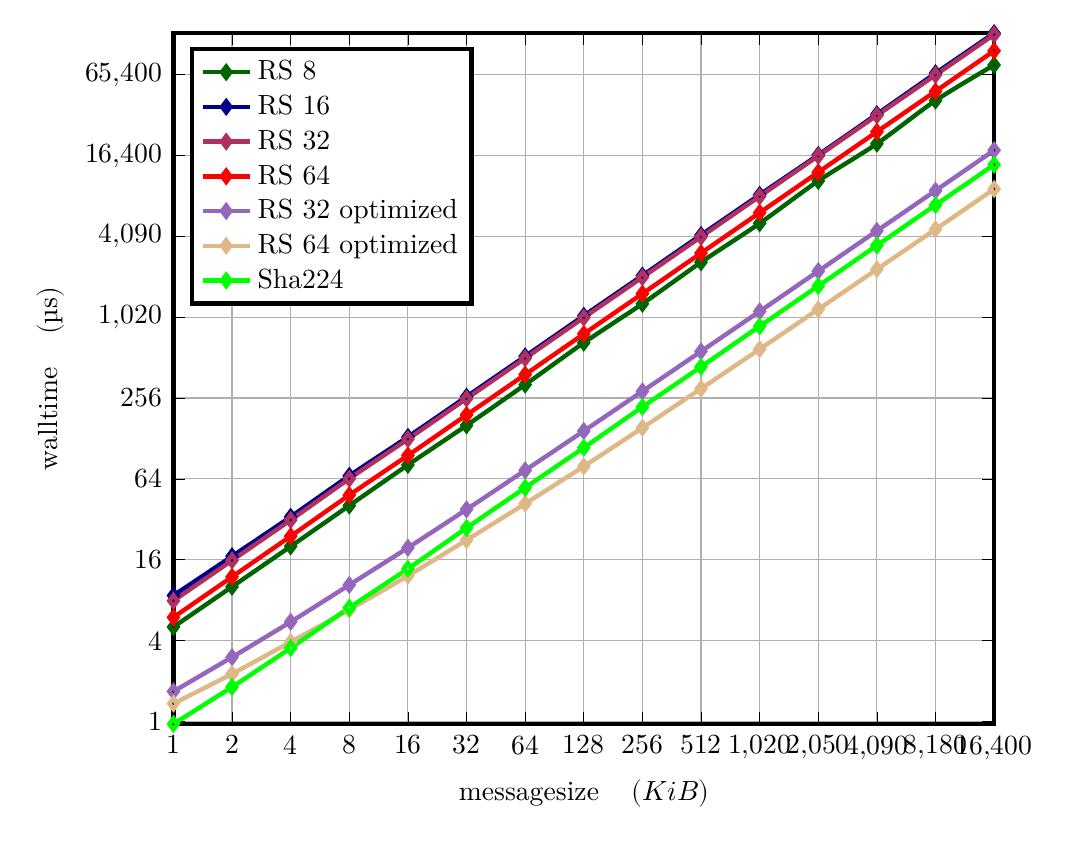
\begin{tikzpicture}
\pgfplotsset{every axis/.append style={ultra thick},compat=1.5}
\definecolor{mycolor0}{rgb}{0.00000, 0.39216, 0.00000}
\definecolor{mycolor1}{rgb}{0.00000, 0.00000, 0.54510}
\definecolor{mycolor2}{rgb}{0.69020, 0.18824, 0.37647}
\definecolor{mycolor3}{rgb}{1.00000, 0.00000, 0.00000}
\definecolor{mycolor4}{rgb}{0.58039, 0.40392, 0.74118}
\definecolor{mycolor5}{rgb}{0.87059, 0.72157, 0.52941}
\definecolor{mycolor6}{rgb}{0.00000, 1.00000, 0.00000}
\definecolor{mycolor7}{rgb}{0.00000, 1.00000, 1.00000}
\definecolor{mycolor8}{rgb}{1.00000, 0.00000, 1.00000}
\definecolor{mycolor9}{rgb}{0.39216, 0.58431, 0.92941}

    \begin{axis}[
        xlabel=$\mathrm{message size}\quad\left(KiB\right)$,
        ylabel=$\mathrm{wall time}\quad\left(\si{\micro\second}\right)$,
        xmajorgrids,
        enlargelimits=false,
        scaled ticks=true,
        ymajorgrids,
        width=0.99*\textwidth,
        log basis x=2,
        % ymin=0,
        % ymax=0,
        % restrict y to domain=0:1,
        log basis y=2,
        xmode=log,
        ymode=log,
        log ticks with fixed point,
        x tick style={color=black},
        y tick style={color=black},
        x grid style={white!69.01960784313725!black},
        y grid style={white!69.01960784313725!black},
        legend style={at={(0.02,0.98)}, anchor=north west,legend cell align=left, align=left},
    ]
\addplot[
        smooth,
        mark=diamond,
        color=mycolor0,
    ] plot coordinates {
            (1,5.05184)
        (2,10.07744)
        (4,20.11882)
        (8,40.46190)
        (16,81.20731)
        (32,159.89795)
        (64,321.52351)
        (128,658.96043)
        (256,1285.47007)
        (512,2617.52278)
        (1024,5101.78212)
        (2048,10546.93570)
        (4096,19967.88823)
        (8192,41786.25591)
        (16384,76925.98503)

    };
    \addlegendentry{RS 8}
    \addplot[
        smooth,
        mark=diamond,
        color=mycolor1,
    ] plot coordinates {
            (1,8.66536)
        (2,16.96434)
        (4,33.37965)
        (8,67.40014)
        (16,131.19935)
        (32,261.51806)
        (64,522.14260)
        (128,1046.11404)
        (256,2083.58617)
        (512,4173.01063)
        (1024,8317.19520)
        (2048,16471.35111)
        (4096,33092.86317)
        (8192,66733.92490)
        (16384,132612.72865)

    };
    \addlegendentry{RS 16}
    \addplot[
        smooth,
        mark=diamond,
        color=mycolor2,
    ] plot coordinates {
            (1,7.91347)
        (2,15.81414)
        (4,31.59336)
        (8,64.11227)
        (16,126.39000)
        (32,252.97787)
        (64,505.36548)
        (128,1013.65463)
        (256,2023.54405)
        (512,4046.96758)
        (1024,8099.29096)
        (2048,16188.66614)
        (4096,32397.46518)
        (8192,64779.96264)
        (16384,129569.89560)

    };
    \addlegendentry{RS 32}
    \addplot[
        smooth,
        mark=diamond,
        color=mycolor3,
    ] plot coordinates {
            (1,5.95841)
        (2,11.93149)
        (4,23.95900)
        (8,48.42613)
        (16,95.59950)
        (32,191.23468)
        (64,381.92467)
        (128,765.97297)
        (256,1528.25669)
        (512,3062.12136)
        (1024,6118.71025)
        (2048,12238.27424)
        (4096,24488.35165)
        (8192,48995.73251)
        (16384,98044.34591)

    };
    \addlegendentry{RS 64}
    \addplot[
        smooth,
        mark=diamond,
        color=mycolor4,
    ] plot coordinates {
            (1,1.67404)
        (2,3.01390)
        (4,5.51860)
        (8,10.38640)
        (16,19.64344)
        (32,37.88738)
        (64,74.02788)
        (128,145.23355)
        (256,286.81980)
        (512,568.13121)
        (1024,1128.40484)
        (2048,2247.45622)
        (4096,4484.49578)
        (8192,8929.22513)
        (16384,17837.37392)

    };
    \addlegendentry{RS 32 optimized}
    \addplot[
        smooth,
        mark=diamond,
        color=mycolor5,
    ] plot coordinates {
            (1,1.35987)
        (2,2.26354)
        (4,3.91345)
        (8,6.79795)
        (16,12.15020)
        (32,22.38704)
        (64,41.80898)
        (128,79.21868)
        (256,153.46299)
        (512,300.09355)
        (1024,590.24875)
        (2048,1168.59667)
        (4096,2319.27543)
        (8192,4600.69073)
        (16384,9177.37798)

    };
    \addlegendentry{RS 64 optimized}
    \addplot[
        smooth,
        mark=diamond,
        color=mycolor6,
    ] plot coordinates {
            (1,0.95956)
        (2,1.80841)
        (4,3.52583)
        (8,7.03387)
        (16,13.70775)
        (32,27.58699)
        (64,54.93119)
        (128,109.07891)
        (256,219.36631)
        (512,436.30522)
        (1024,874.86650)
        (2048,1743.39918)
        (4096,3491.41355)
        (8192,6978.88027)
        (16384,13935.58300)

    };
    \addlegendentry{Sha224}
     
    \end{axis}
    \end{tikzpicture}       
    
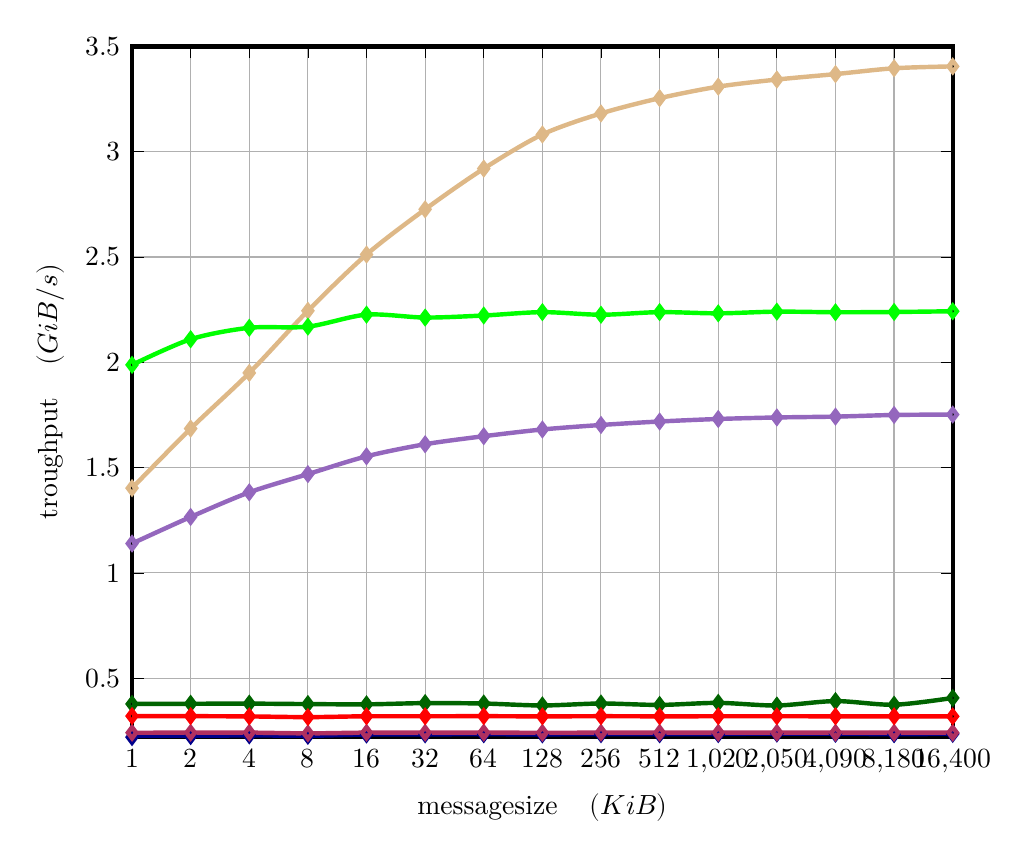
\begin{tikzpicture}
\pgfplotsset{every axis/.append style={ultra thick},compat=1.5}
\definecolor{mycolor0}{rgb}{0.00000, 0.39216, 0.00000}
\definecolor{mycolor1}{rgb}{0.00000, 0.00000, 0.54510}
\definecolor{mycolor2}{rgb}{0.69020, 0.18824, 0.37647}
\definecolor{mycolor3}{rgb}{1.00000, 0.00000, 0.00000}
\definecolor{mycolor4}{rgb}{0.58039, 0.40392, 0.74118}
\definecolor{mycolor5}{rgb}{0.87059, 0.72157, 0.52941}
\definecolor{mycolor6}{rgb}{0.00000, 1.00000, 0.00000}
\definecolor{mycolor7}{rgb}{0.00000, 1.00000, 1.00000}
\definecolor{mycolor8}{rgb}{1.00000, 0.00000, 1.00000}
\definecolor{mycolor9}{rgb}{0.39216, 0.58431, 0.92941}
    \begin{axis}[
        xlabel=$\mathrm{message size}\quad\left(KiB\right)$,
        ylabel=$\mathrm{troughput}\quad\left(GiB/s\right)$,
        width=0.99*\textwidth,
        xmajorgrids,
        enlargelimits=false,
        scaled ticks=true,
        ymajorgrids,
        log basis x=2,
        xmode=log,
		ymax=3.5,
        log ticks with fixed point,
        x tick style={color=black},
        y tick style={color=black},
        x grid style={white!69.01960784313725!black},
        y grid style={white!69.01960784313725!black},
]
\addplot[
        smooth,
        mark=diamond,
        color=mycolor0,
    ] plot coordinates {
            (1,0.37756)
        (2,0.37854)
        (4,0.37922)
        (8,0.37711)
        (16,0.37580)
        (32,0.38171)
        (64,0.37966)
        (128,0.37049)
        (256,0.37985)
        (512,0.37309)
        (1024,0.38283)
        (2048,0.37037)
        (4096,0.39125)
        (8192,0.37393)
        (16384,0.40623)

    };
    \addplot[
        smooth,
        mark=diamond,
        color=mycolor1,
    ] plot coordinates {
            (1,0.22011)
        (2,0.22487)
        (4,0.22856)
        (8,0.22639)
        (16,0.23260)
        (32,0.23339)
        (64,0.23379)
        (128,0.23338)
        (256,0.23435)
        (512,0.23402)
        (1024,0.23483)
        (2048,0.23715)
        (4096,0.23608)
        (8192,0.23414)
        (16384,0.23565)

    };
    \addplot[
        smooth,
        mark=diamond,
        color=mycolor2,
    ] plot coordinates {
            (1,0.24103)
        (2,0.24122)
        (4,0.24149)
        (8,0.23800)
        (16,0.24146)
        (32,0.24127)
        (64,0.24155)
        (128,0.24085)
        (256,0.24130)
        (512,0.24131)
        (1024,0.24115)
        (2048,0.24130)
        (4096,0.24115)
        (8192,0.24120)
        (16384,0.24118)

    };
    \addplot[
        smooth,
        mark=diamond,
        color=mycolor3,
    ] plot coordinates {
            (1,0.32011)
        (2,0.31972)
        (4,0.31844)
        (8,0.31509)
        (16,0.31922)
        (32,0.31916)
        (64,0.31962)
        (128,0.31873)
        (256,0.31950)
        (512,0.31892)
        (1024,0.31921)
        (2048,0.31918)
        (4096,0.31903)
        (8192,0.31891)
        (16384,0.31873)

    };
    \addplot[
        smooth,
        mark=diamond,
        color=mycolor4,
    ] plot coordinates {
            (1,1.13937)
        (2,1.26570)
        (4,1.38249)
        (8,1.46911)
        (16,1.55358)
        (32,1.61096)
        (64,1.64898)
        (128,1.68102)
        (256,1.70240)
        (512,1.71890)
        (1024,1.73087)
        (2048,1.73808)
        (4096,1.74211)
        (8192,1.74987)
        (16384,1.75194)

    };
    \addplot[
        smooth,
        mark=diamond,
        color=mycolor5,
    ] plot coordinates {
            (1,1.40260)
        (2,1.68528)
        (4,1.94953)
        (8,2.24462)
        (16,2.51169)
        (32,2.72636)
        (64,2.91972)
        (128,3.08186)
        (256,3.18175)
        (512,3.25419)
        (1024,3.30899)
        (2048,3.34268)
        (4096,3.36851)
        (8192,3.39623)
        (16384,3.40511)

    };
    \addplot[
        smooth,
        mark=diamond,
        color=mycolor6,
    ] plot coordinates {
            (1,1.98774)
        (2,2.10942)
        (4,2.16385)
        (8,2.16933)
        (16,2.22630)
        (32,2.21246)
        (64,2.22224)
        (128,2.23820)
        (256,2.22587)
        (512,2.23826)
        (1024,2.23248)
        (2048,2.24059)
        (4096,2.23763)
        (8192,2.23890)
        (16384,2.24246)

    };
     
    \end{axis}
    \end{tikzpicture}       
    
\end{figure}
\begin{figure}
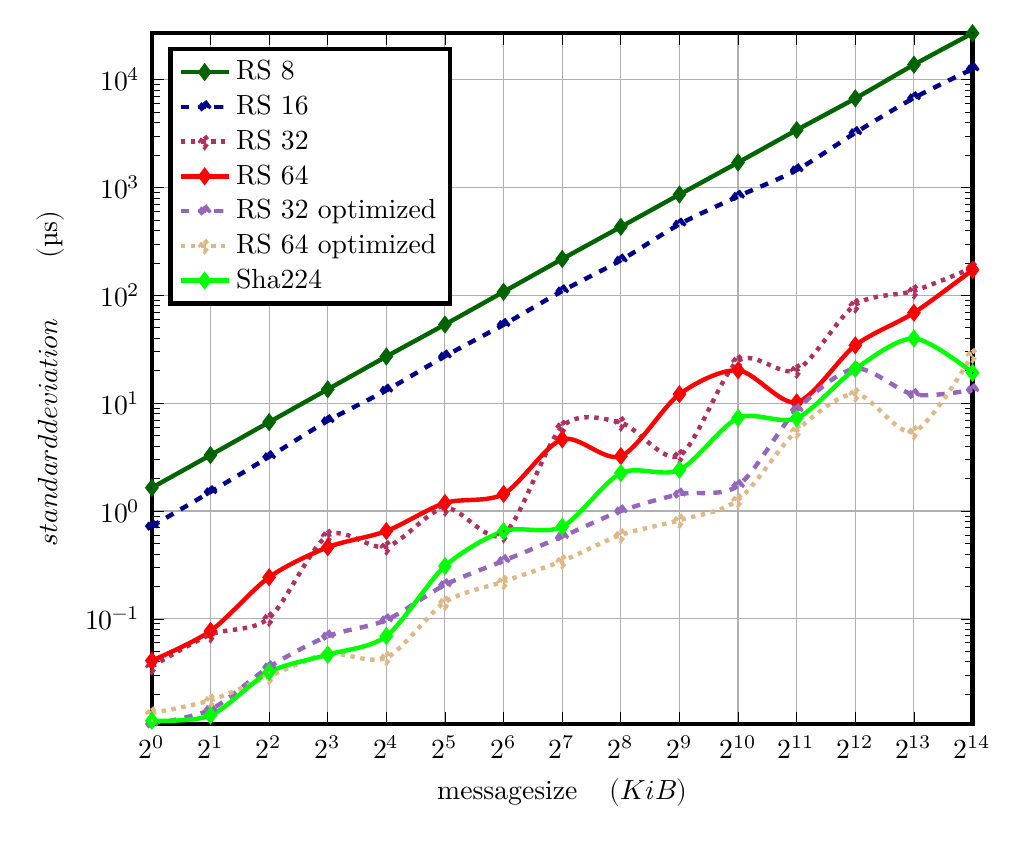
\begin{tikzpicture}
\pgfplotsset{every axis/.append style={ultra thick},compat=1.5}\definecolor{mycolor0}{rgb}{0.00000, 0.39216, 0.00000}
\definecolor{mycolor1}{rgb}{0.00000, 0.00000, 0.54510}
\definecolor{mycolor2}{rgb}{0.69020, 0.18824, 0.37647}
\definecolor{mycolor3}{rgb}{1.00000, 0.00000, 0.00000}
\definecolor{mycolor4}{rgb}{0.58039, 0.40392, 0.74118}
\definecolor{mycolor5}{rgb}{0.87059, 0.72157, 0.52941}
\definecolor{mycolor6}{rgb}{0.00000, 1.00000, 0.00000}
\definecolor{mycolor7}{rgb}{0.00000, 1.00000, 1.00000}
\definecolor{mycolor8}{rgb}{1.00000, 0.00000, 1.00000}
\definecolor{mycolor9}{rgb}{0.39216, 0.58431, 0.92941}
    \begin{axis}[
        xlabel=$\mathrm{message size}\quad\left(KiB\right)$,
        ylabel=$standard deviation\quad\quad\left(\si{\micro\second}\right)$,
        width=0.99*\textwidth,
        xmajorgrids,
        enlargelimits=false,
        scaled ticks=true,
        ymajorgrids,
        log basis x=2,
        xmode=log,
        x tick style={color=black},
        y tick style={color=black},
        ymode=log,
        x grid style={white!69.01960784313725!black},
        y grid style={white!69.01960784313725!black},
        legend style={at={(0.02,0.98)}, anchor=north west,legend cell align=left, align=left},
]
\addplot[
        smooth,
        mark=diamond,
        color=mycolor0,
    ] plot coordinates {
            (1,1.64305)
        (2,3.29604)
        (4,6.66578)
        (8,13.42416)
        (16,27.04653)
        (32,53.59396)
        (64,107.71159)
        (128,216.97769)
        (256,431.05438)
        (512,859.46286)
        (1024,1704.02760)
        (2048,3407.52702)
        (4096,6697.89500)
        (8192,13744.89314)
        (16384,26924.79770)

    };
    \addlegendentry{RS 8}
    \addplot[
        smooth,
        mark=diamond,
        dashed,
        color=mycolor1,
    ] plot coordinates {
            (1,0.72356)
        (2,1.50358)
        (4,3.17781)
        (8,6.84917)
        (16,13.14705)
        (32,27.23173)
        (64,53.42111)
        (128,109.63277)
        (256,211.50810)
        (512,455.55236)
        (1024,826.25997)
        (2048,1451.40683)
        (4096,3212.25626)
        (8192,6757.65181)
        (16384,12531.38377)

    };
    \addlegendentry{RS 16}
    \addplot[
        smooth,
        mark=diamond,
        dotted,
        color=mycolor2,
    ] plot coordinates {
            (1,0.03616)
        (2,0.07140)
        (4,0.10165)
        (8,0.59303)
        (16,0.46559)
        (32,1.06972)
        (64,0.60633)
        (128,6.07127)
        (256,6.57666)
        (512,3.26110)
        (1024,24.62322)
        (2048,20.28439)
        (4096,81.75853)
        (8192,109.90583)
        (16384,179.81963)

    };
    \addlegendentry{RS 32}
    \addplot[
        smooth,
        mark=diamond,
        solid,
        color=mycolor3,
    ] plot coordinates {
            (1,0.04096)
        (2,0.07717)
        (4,0.24294)
        (8,0.46103)
        (16,0.65129)
        (32,1.18662)
        (64,1.43872)
        (128,4.61606)
        (256,3.22151)
        (512,12.10471)
        (1024,20.13524)
        (2048,10.18716)
        (4096,34.35261)
        (8192,68.85330)
        (16384,172.05282)

    };
    \addlegendentry{RS 64}
    \addplot[
        smooth,
        mark=diamond,
        dashed,
        color=mycolor4,
    ] plot coordinates {
            (1,0.01060)
        (2,0.01439)
        (4,0.03573)
        (8,0.06895)
        (16,0.09750)
        (32,0.20639)
        (64,0.34530)
        (128,0.57816)
        (256,0.99852)
        (512,1.43079)
        (1024,1.71639)
        (2048,8.66373)
        (4096,20.91269)
        (8192,11.99794)
        (16384,13.27155)

    };
    \addlegendentry{RS 32 optimized}
    \addplot[
        smooth,
        mark=diamond,
        dotted,
        color=mycolor5,
    ] plot coordinates {
            (1,0.01335)
        (2,0.01758)
        (4,0.02928)
        (8,0.04728)
        (16,0.04366)
        (32,0.14249)
        (64,0.22168)
        (128,0.34375)
        (256,0.59938)
        (512,0.82183)
        (1024,1.26600)
        (2048,5.55672)
        (4096,12.17414)
        (8192,5.42795)
        (16384,28.10881)

    };
    \addlegendentry{RS 64 optimized}
    \addplot[
        smooth,
        mark=diamond,
        solid,
        color=mycolor6,
    ] plot coordinates {
            (1,0.01136)
        (2,0.01271)
        (4,0.03207)
        (8,0.04650)
        (16,0.06917)
        (32,0.30791)
        (64,0.64978)
        (128,0.71403)
        (256,2.24559)
        (512,2.40309)
        (1024,7.29453)
        (2048,7.24790)
        (4096,20.76392)
        (8192,39.79086)
        (16384,19.11556)

    };
    \addlegendentry{Sha224}
     
    \end{axis}
    \end{tikzpicture}       
    
\end{figure}
\newpage

\section{Conclusion and Outlook}

The presented optimized 32 bit and 64 bit RS encoder can reach speeds similar to Sha224 while simultaneously allowing much larger message/world sizes. This makes RS encoders viable for practical used.

The approach presented here is of particular interest to embedded use cases and custom hardware. A carryless multiplication can be implemented more easily and with less area requirements compared to a dedicated Sha2 encoder. Even compared to a conventional multiplier less area is required as all adders can be replaced with simple XOR gates. An existing multiplier  could even be reused by adding a flag that controls whether carrys are considered.

Future work could focus on also accelerating smaller symbol sizes like 8 bit and 16 bit with CLMU instructions. To that end multiple 8bit/16bit multiplications could be performed with a single (64bit) CLMU instruction. The use of smaller symbol sizes would further reduce network traffic at he cost of increased collision rate. 

Furthermore, future work  could investigate the impact of the chosen modulus polynomial on false positive rates. Exiting literature has established the choice of modulus polynomial affects how often and what kind of errors are detected~\cite{Jones2009}. Similar concerns likely apply to RS-ID codes too.

\printbibliography
\end{document}
